\section{Data Sources and Preprocessing}
\label{sec:data}
MindDrifter is constructed from English Wikipedia. We will refer to it as Wiki 
from this point on.
% MindDrifter is constructed from three data sources: Chinese Wikipedia,
% Baidu Encyclopedia and Hudong Encyclopedia. We will refer to these
% sources as Wiki, Baidu and Hudong from this point on.
Each article in the data source is 
a unit for processing. The snapshots of Wiki, which
we use in this paper were crawled directly from the web in 2014,
and contain 4 million pages and 1 million categories.
All articles in the data source are contributed by community	
authors. Each article has a title which is either a concept or an entity,
and a body text with hyperlinks to other pages to describe the title.
\figref{fig:wikipage} shows the pages for ``David Beckham'' in Wiki, Baidu
and Hudong.

\begin{figure*}[th]
\centering
%\epsfig{file=wikipage.eps,width=1.4\columnwidth}
\epsfig{file=wikipage1.eps,width=1.8\columnwidth}
\caption{Snapshots of Wiki, Baidu and Hudong Pages}
\label{fig:wikipage}
\shrink
\end{figure*}

We extract four types of information
from a page: the {\em outgoing links} to other pages which helps us
construct a link graph from all pages;
the {\em labels} of each page, which helps us 
figure out the context of the page, 
%JY{title-body, sentence-level, title-link, category} 
{\em title-body co-occurrence} (or TB for short)
which measures the number of times a term
occurs in a page under a title;
and finally, {\em sentence-level co-occurrence} (or SL for short),
representing the co-occurrence of two terms within one sentence in any page.
These four type of information play different roles and hence have different
significance.

The outgoing links represent the potential change of topics,
i.e., jumping from a page of a certain topic to a page of a different topic.
The topics are known as {\em contexts} here and
example of contexts include ``people'', ``nature'', ``technology'',
``sports'', etc. The processing of clicking an outgoing
link to enter a different page is known as {\em context transition}
in this paper. Note that the new page maybe on the same topic or context,
in which case, the user remains in the same context, or in other word, it is
a self transition. We use this information to compute a transition matrix
between contexts from the whole data.

On the other hand, we consider TB co-occurrence and SL co-occurrence
to represent relatedness in two orthogonal dimensions.
The TB co-occurrence represents relatedness in a ``vertical'' direction,
that is, one concept is part or a feature of the other concept,
or one concept is a generalization of the other concept.
The association from ``football'' to
``David Beckham" and that from ``Victoria Beckham'' to ``Spice Girls''
are examples of such vertical relatedness.
Whereas SL co-occurrence gives the relatedness in horizontal direction,
that is,  two concepts which have close relation and work together to
represent some more complex meaning.
The association from ``David Beckham'' to ``Victoria Beckham'' falls
into this category.
We further conjecture that when people makes a one-step association
from a given concept, they either drift their mind vertically or horizontally,
each direction with a prior probability. The ratio between these two
probabilities differs from context to context.
In \secref{sec:approach} we will introduce how we learn the ratio
as a parameter called $\alpha$, and use it to combine the
two types of co-occurrences together.

In Baidu and Hudong, a page may contain a number of sections, each of
which describing a different entity of the same title. For example,
apple the computer and apple the fruit are in the same Baidu or Hudong page.
In other words, a Baidu or a Hudong page contains all information
about a {\em term} and not a {\em sense} of a term. This is different in
Wiki which distinguish different senses of the same term, so that
apple the computer and apple the fruit each have its own page.
In this work, we merge the different pages under the same surface form in Wiki
to form a ``master page'' just like Baidu and Hudong.
Many articles in three data sources share the same title.
For example, all three encyclopedias have a page (or a master page)
about ``apple.'' These three page are usually different in content.
We again merge these pages to form a ``super page'' about apple.
%We first count
%the number of links and those two types of co-occurrence in each data source
%separately, and then merge the two types of co-occurrences in three sources
%together.
Subsequently, we obtain a link graph among all the super pages \footnote{An
ordinary page whose title is not found in other sources is not merged
with other pages but is also called a ``super page''.}
and compute TB co-occurrences and SL co-occurrences in terms of these
super pages.

In addition, there are synonyms in the merged dataset.
We find out synonyms from the page-redirection information
in the three online encyclopedia, and linked those synonyms to a synset.
%\KZ{How do we determine synsets and link them together?}
Each synset has a representative title
and a list of terms which are the synonymous to the representative title.
We merge the co-occurrences related to terms in the same synset as well.
In the end, the TB and SL co-occurrences are essentially computed between
synsets in the merged dataset.

%\KZ{Add algo for clustering and merging, and add some discussion in the text.}
We conjecture that people will associate differently under different context,
all the data are collected within its context. We assume the information in
a super page is under the same context, and the labels of the page
(shown in \figref{fig:wikipage})
can represent these context. Thus all the TB co-occurrence and SL
co-occurrence collected in this super page are under the same context.
To reduce the complexity for practical reason,
and to get more typical context, we cluster all the labels into
several clusters of contexts,
each of which focuses on a relatively independent topic.
Since each page has several labels, and these labels might belong
to some contexts, we can refer a page to these contexts
its labels belong to.

We use revised $k$-medoids algorithm to do label clustering.
To get a better clustering result,
we first manually select $k$ typical labels as the initial centers for
the $k$ clusters, and then use the page-label information to
compute the distance between two pages.
To be specific, each page has several labels, and correspondingly,
each label was used to label several pages, then we can use
the overlap of the pages under two labels to calculate their
relatedness. The relatedness for label $a$ and $b$ is calculated as follows:

\begin{equation}
R(a,b)=\frac{N(overlap(P_a,P_b))}{N(P_a)+N(P_b)-N(overlap(P_a,P_b))}
\end{equation}
where $P_a$ is a set of encyclopedia pages that use $a$ as labels,
$N(P_a)$ is the number of pages in set $P_a$, and $N(overlap(P_a,P_b))$
is the number of the overlap pages in the two sets.
